\synctex=1
\documentclass{beamer}
%
% Choose how your presentation looks.
%
% For more themes, color themes and font themes, see:
% http://deic.uab.es/~iblanes/beamer_gallery/index_by_theme.html
%
\mode<presentation>
{
  \usetheme{default}      % or try Darmstadt, Madrid, Warsaw, ...
  \usecolortheme{default} % or try albatross, beaver, crane, ...
  \usefonttheme{default}  % or try serif, structurebold, ...
  \setbeamertemplate{navigation symbols}{}
  \setbeamertemplate{caption}[numbered]
} 

\usepackage[english]{babel}
\usepackage[utf8x]{inputenc}
\usepackage{graphicx}
\usepackage{amsmath}

\title[Simuladores de Conducción]{Simuladores de Conducción para vehículos Terrestres}
\author{José González Moya}
\institute{Universidad Andrés Bello}
\date{5 Diciembre 2018}

\begin{document}

\begin{frame}
  \titlepage
\end{frame}

% Uncomment these lines for an automatically generated outline.
%\begin{frame}{Outline}
%  \tableofcontents
%\end{frame}

\section{Introducción}

\begin{frame}{Introducción}

\begin{itemize}
  \item En el centro de modelación y simulación del ejército, existe un creciente desarrollo de simuladores de conducción.
  \item Proyecto Fondecyt, entre el CEMSE y la universidad católica, en el año 2011.
  \item Sofware Padrob, desarrollado por la Universidad Católica.
  \item CEMSE cuenta con el simulador de camión UNIMOG. Éste tiene sensores para medir presión, temperatura, y un sistema de adquisición de datos.
  \item Actualmente el simulador es estático, no trata de simular sensaciones de conducción.
\end{itemize}

\vskip 1cm

%\begin{block}{Examples}
%Some examples of commonly used commands and features are included, to help you get started.
%\end{block}
\end{frame}

\section{Simulador y Software}

\begin{frame}{Simulador y Software}

\begin{figure}[h]
\centering
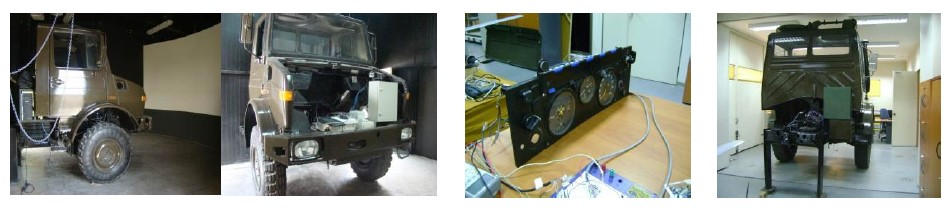
\includegraphics[scale=0.4]{Unimog_1300}
%\caption{unimog1}

\end{figure}

\begin{figure}[h]
\centering
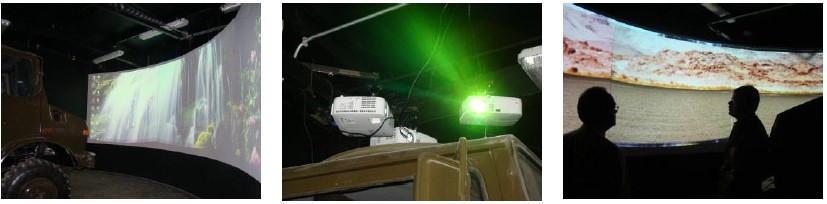
\includegraphics[scale=0.4]{simulador_software}
%\caption{unimog1}

\end{figure}


\vskip 1cm
\end{frame}



\section{Motivación}

\begin{frame}{Motivación}

\begin{itemize}
 \item Proponer e investigar acerca de un sistema robótico para resolver el problema de verosimilitud.
 \item Modelar matemáticamente un sistema vehicular.
\end{itemize}
\vskip 1cm
\end{frame}

\section{Objetivos}

\begin{frame}{Objetivos}
\begin{block}{Objetivo General del trabajo} Simular las sensaciones que experimenta un conductor, cómo sensaciones de aceleración, frenados repentinos, o virajes bruscos, también puede simular las irregularidades del terreno, pantanoso montañoso, etc.
\end{block}
\begin{block}{Objetivos Especificos}
\begin{itemize}
 \item Resolver la cinemática inversa de la plataforma Stewart.
 \item Modelar sistemas de suspensión del vehículo.
 \item Modelar un vehículo en 2D, que se desplaza por una superficie arbitraria.
 \item Integrar los modelos en un simulador que permita alcanzar el objetivo general.
\end{itemize}
\end{block}

\end{frame}

\begin{frame}{Esquema de la presentación}

\begin{itemize}
 \item Plataforma Stewart y cinemática Inversa.
 \item Modelos de suspensión Quarter-Car.
 \item Modelo de vehículo simplificado en 2D. 
 \item Modelo de vehículo simplificado 2D en un camino arbitrario $y=f(x)$.
\end{itemize}
\vskip 1cm
\end{frame}
\begin{frame}{Plataforma Stewart}

\begin{itemize}
 \item La plataforma Stewart es un sistema robótico.
 \item Se usa en simuladores de vuelo  y de conducción.
 
\begin{figure}[h]
\centering
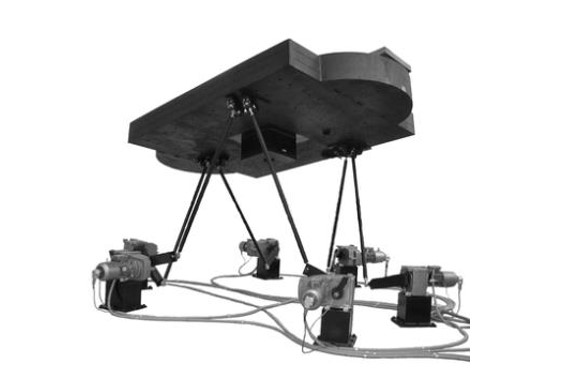
\includegraphics[scale=0.4]{stewart}
%\caption{unimog1}

\end{figure}
 
\end{itemize}
\vskip 1cm
\end{frame}
\section{Plataforma Stewart}
\begin{frame}{Plataforma Stewart: modelo geométrico}

 \begin{figure}[h]
\centering
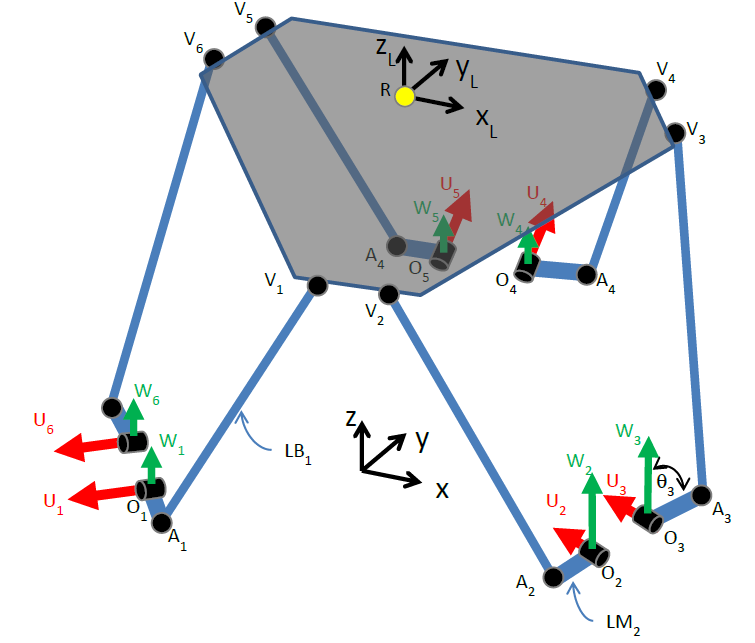
\includegraphics[scale=0.35]{plataform_stewart}
%\caption{unimog1}

\end{figure}
\vskip 1cm
\end{frame}

\section{Plataforma Stewart}
\begin{frame}{Cinemática Inversa}
\begin{figure}[h]
\centering
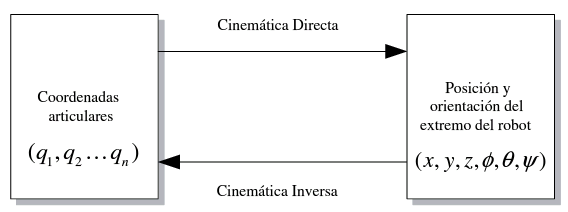
\includegraphics[scale=0.4]{cinematica}
%\caption{unimog1}

\end{figure}
\begin{figure}[h]
\centering
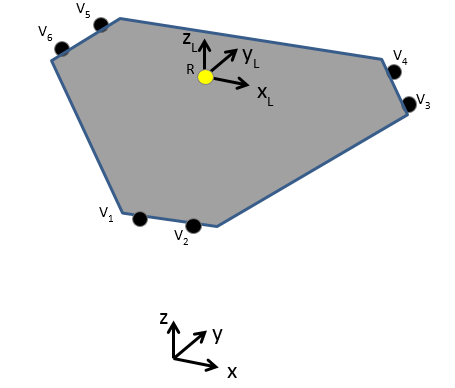
\includegraphics[scale=0.35]{base_sup}
%\caption{unimog1}

\end{figure}

\end{frame}

%\subsection{Mathematics}

\begin{frame}{Cinématica Inversa: Planteo matemático del problema}
Luego el sistema de ecuaciones no lineales que hay que resolver es el siguiente
$$(A_{ix}-O_{ix})^{2}+(A_{iy}-O_{iy} )^{2}+(A_{iz}-O_{iz})^{2} = LM_{i}^{2}$$
\end{frame}


\section{Plataforma Stewart}
\begin{frame}{Resultados Gráficos de la plataforma y Animación}
\begin{center}
\begin{tabular}{cc}
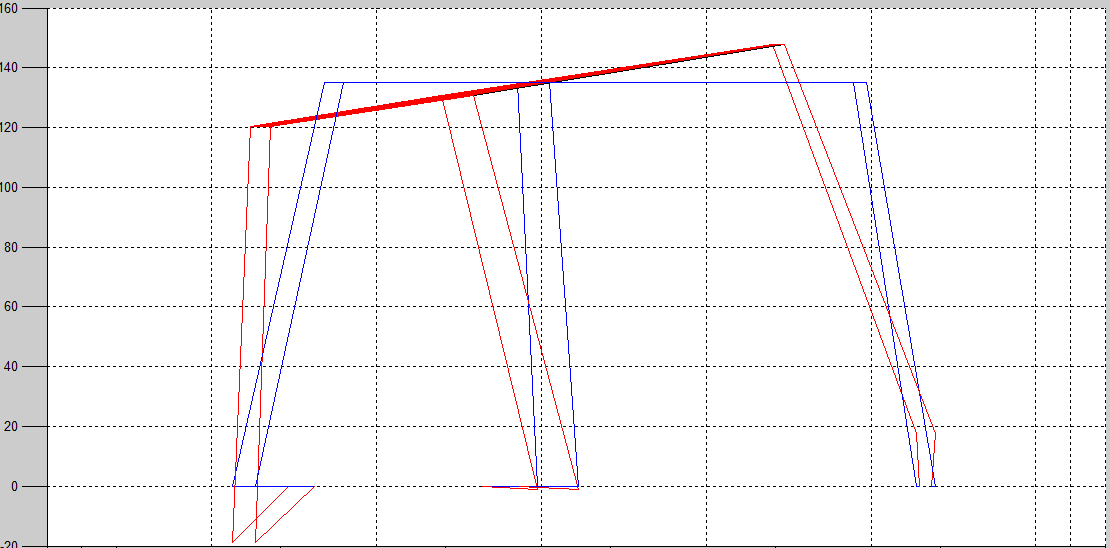
\includegraphics[scale=0.15]{10grados}&
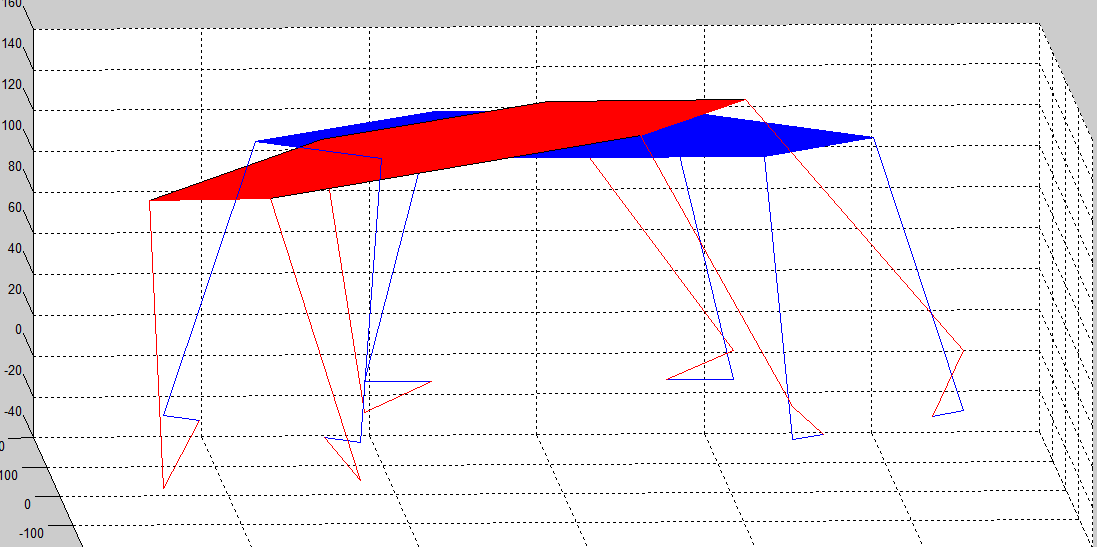
\includegraphics[scale=0.15]{15grados}\\
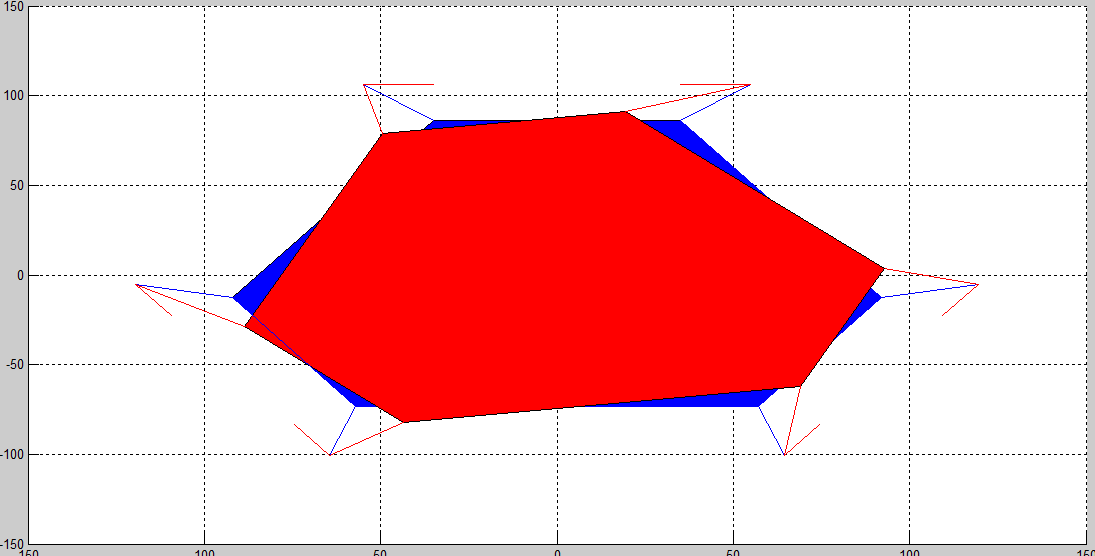
\includegraphics[scale=0.15]{rol}&
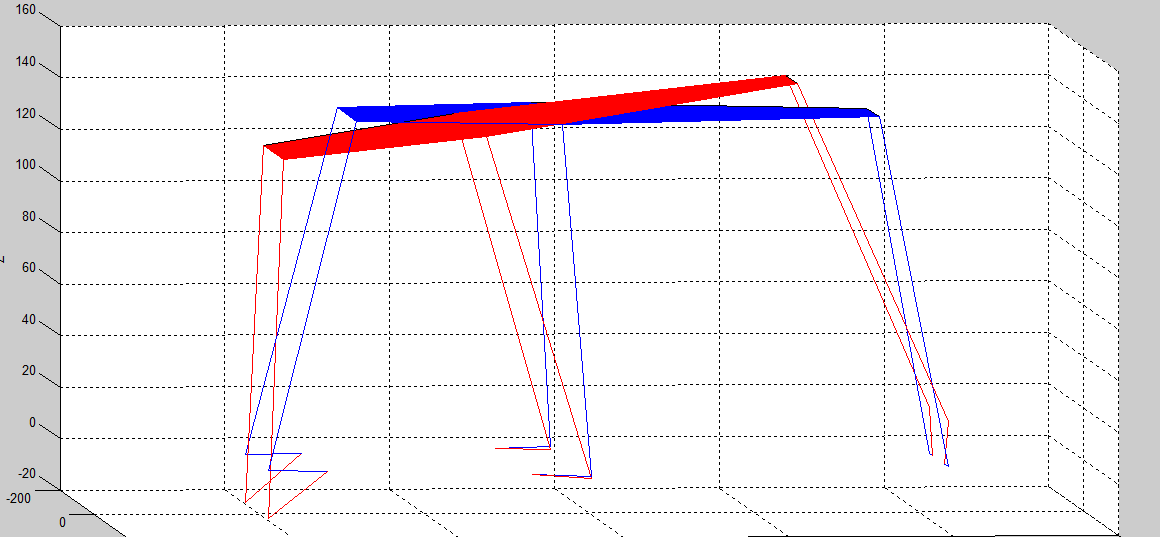
\includegraphics[scale=0.15]{10gradosotra}
\end{tabular}
\end{center}

\vskip 1cm
\end{frame}

\section{Modelo 2D}
\begin{frame}{Modelo de vehículo 2D}
 \begin{figure}[h]
\centering
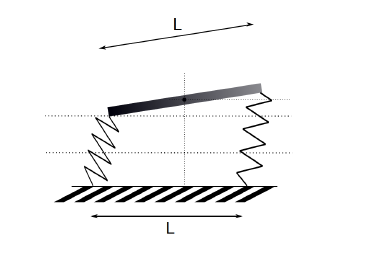
\includegraphics[scale=0.35]{resortes}
%\caption{unimog1}

\end{figure}

\vskip 1cm
\end{frame}

\section{Quarter-Car}
\begin{frame}{Modelo 2D--Lagrangeano del sistema}
El Lagrangiano está dado por
\begin{multline*}
L(x,y,\theta,\dot x,\dot y,\dot \theta)= \frac{1}{2}m(\dot x^2 +  \dot y^2)+ \frac{1}{2} I_{cm} \dot \theta^2-mgy\\
-\frac{1}{2}k(\Delta l_{1}-l_{0})^2-\frac{1}{2}k(\Delta l_{2}-l_{0})^2 
\end{multline*}
con 
\begin{eqnarray*}
\Delta x_{1} = \frac{L}{2}+ x - \frac{L}{2} \cos(\theta) \\ 
\Delta y_{1} =   y +  y_{0} - \frac{L}{2}  \sin(\theta) \\ 
\Delta x_{2} = x + \frac{L}{2}  \cos(\theta)-\frac{L}{2}\\ 
\Delta l_{1} = \sqrt  {\Delta x_{1}^2+ \Delta y_{1}^2} %= \sqrt{(\frac{L}{2}+ x - \frac{L}{2}  \cos(\theta))^2+ (y+y_{0} - \frac{L}{2}  \sin(\theta))^2}
\\ 
\Delta l_{2} =  \sqrt  {\Delta x_{2}^2+ \Delta y_{2}^2}
\end{eqnarray*}
%Aplicamos la ecuación de Euler--Lagrange:

%$$\frac{d}{dt}\left(\frac{\partial L} {\partial \dot x}\right) = \frac{\partial L}%{\partial x}$$
%para obtener las ecuaciones de movimiento...
\end{frame}
\begin{frame}{Ecuaciones de Movimiento}

  \begin{eqnarray*}
  m\ddot x  & = & -k \Delta x_{1} (1 - \frac {l_{0}}{\Delta l_{1}}) - k \Delta x_{2} (1-\frac {l_{0}}{\Delta l_{2}})   
  \\m\ddot y  & =&  -k \Delta y_{1} (1 - \frac {l_{0}}{\Delta l_{1}}) - k \Delta y_{2} (1-\frac {l_{0}}{\Delta l_{2}}) - mg
  \\I_{cm}\ddot \theta  & = &  -\frac{k}{2}[L\sin(\theta) \Delta x_{1} L\cos(\theta) \Delta y_{1}][1- \frac{l_{0}}{\Delta l_{1}}]\\
 & &  -\frac{k}{2}[L\cos(\theta)\Delta y_{2}-L \sin(\theta)\Delta x_{2} ][1- \frac{l_{0}}{\Delta l_{2}}]  
  \end{eqnarray*}
  
\end{frame}
\section{Modelo 2D}
\begin{frame}{Animaciones}
%Animaciones
\vskip 1cm
\end{frame}

\section{Quarter-CAR}
\begin{frame}{Suspensión Quarter-Car}
\begin{figure}[h]
\centering
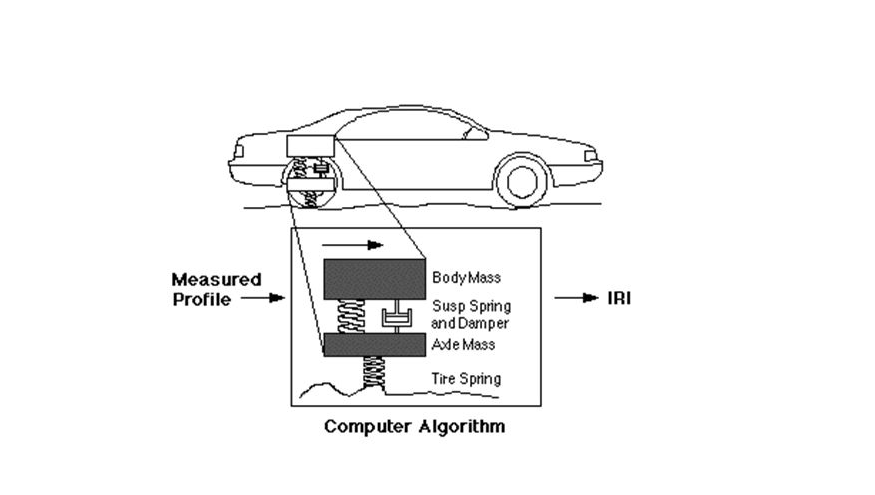
\includegraphics[scale=0.35]{quarter_susp}
%\caption{unimog1}

\end{figure}
\end{frame}

\begin{frame}{Suspensión Quarter-Car}
 \begin{figure}[h]
\centering
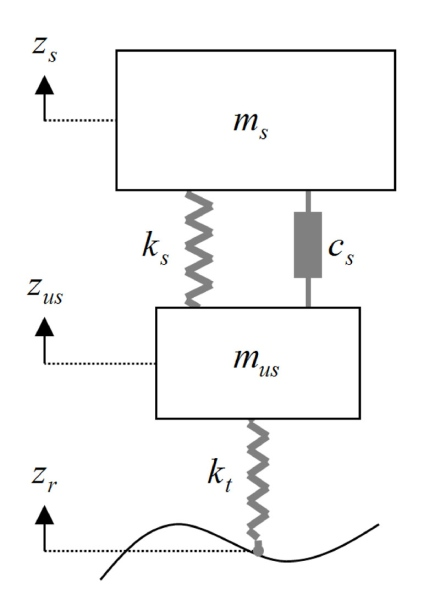
\includegraphics[scale=0.35]{quarter-car}
%\caption{unimog1}

\end{figure}

\vskip 1cm
\end{frame}

\section{Ecuaciones de movimiento quarter car}
\begin{frame}{Ecuaciones de Movimiento Quarter-Car}
\begin{align*}
L(z_{s},z_{us},\dot z_{s},\dot z_{us}) & = \frac{1}{2} m_{s} \dot z_{s}^2 + \frac{1}{2} m_{us} \dot z_{us}^2 -\frac{1}{2} k_{t}(z_{us}-z_{r}(t))^2 -\frac{1}{2} k_{s}(z_{s}-z_{us})^2
\end{align*}
Luego la primera ecuación de Euler Lagrange
$$\frac{d}{dt}\left(\frac{\partial L} {\partial \dot z_{s}}\right) - \frac{\partial L}{\partial z_{s}} = Q_{z_{s}}$$
La primera ecuación de movimiento
$$\ddot z_{s} = -\frac {k_{s}}{m_{s}} (z_{s} - z_{us}) - \frac {c_{s}}{m_{s}} (\dot z_{s} - \dot z_{us})$$ 
La segunda Ecuación de Euler Lagrange está dada por
$$\frac{d}{dt}\left(\frac{\partial L} {\partial \dot z_{us}}\right) - \frac{\partial L}{\partial z_{us}} = Q_{z_{us}}$$
Luego la segunda ecuación de movimiento está dada por
\begin{align*}
\ddot z_{us} &= \frac {k_{s}}{m_{us}} (z_{s} - z_{us}) - \frac {k_{t}}{m_{us}}(z_{us}-z_{r}(t)) + \frac{c_{s}}{m_{us}} (\dot z_{s} - \dot z_{us})
\end{align*}

El sistema de ecuaiones diferenciales
\begin{align*}
\ddot z_{us} &= \frac {k_{s}}{m_{us}} (z_{s} - z_{us}) - \frac {k_{t}}{m_{us}}(z_{us}-z_{r}(t)) + \frac{c_{s}}{m_{us}} (\dot z_{s} - \dot z_{us})  \\
\ddot z_{s}  &= -\frac {k_{s}}{m_{s}} (z_{s} - z_{us}) - \frac {c_{s}}{m_{s}} (\dot z_{s} - \dot z_{us})
\end{align*}
\vskip 1cm
\end{frame}

\section{Modelo 2D}
\begin{frame}{Resultados Quarter-Car}

 \begin{figure}[h]
\centering
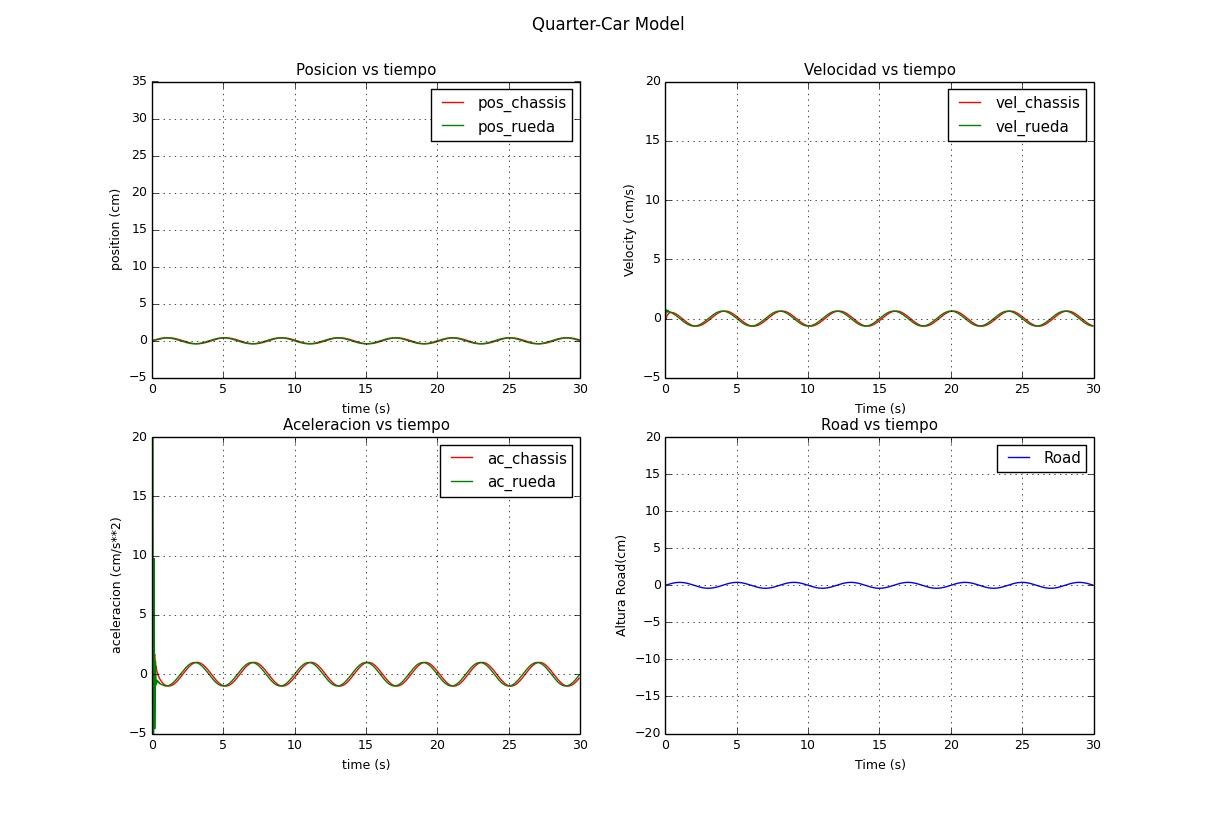
\includegraphics[scale=0.35]{1_resorte}
%\caption{unimog1}

\end{figure}
\begin{figure}[h]
\centering
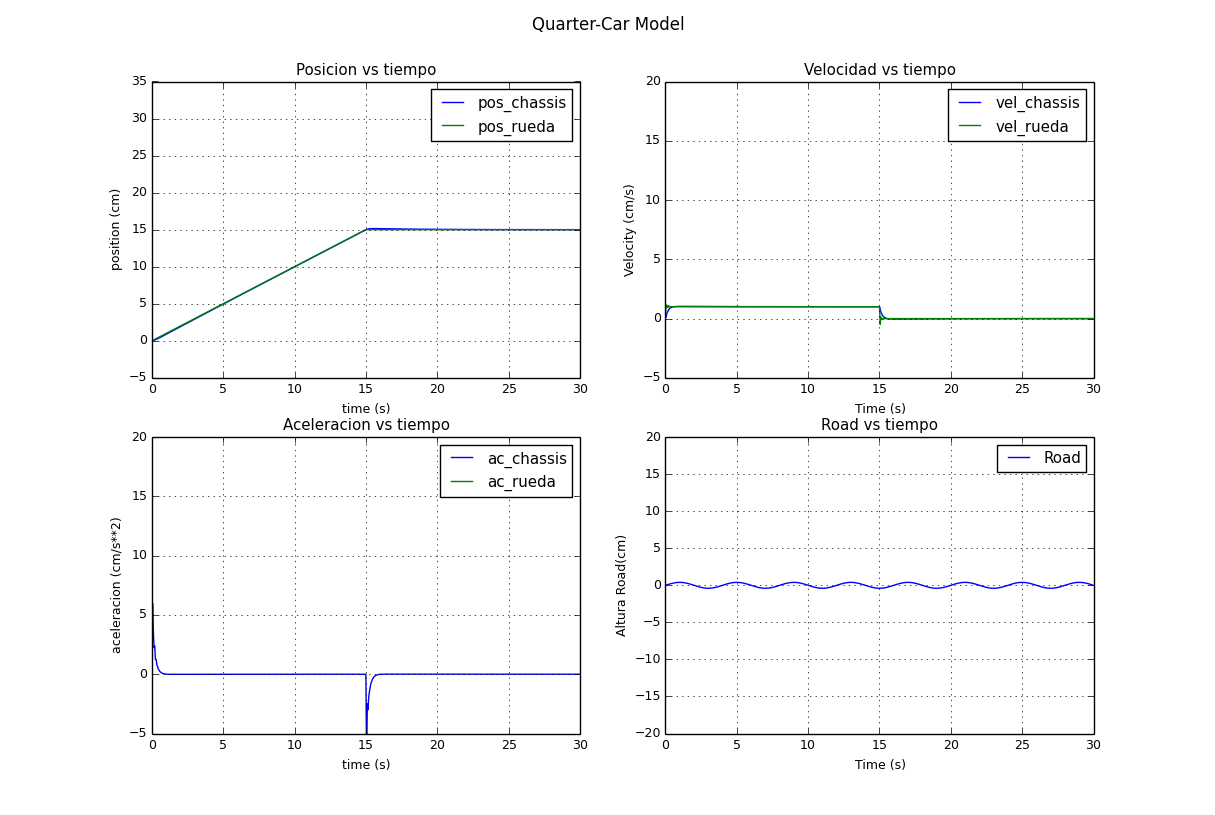
\includegraphics[scale=0.35]{quarter_sim_pendiente}
%\caption{unimog1}

\end{figure}

\vskip 1cm
\end{frame}

\section{Modelo 2D}
\begin{frame}{Conclusiones}
\begin{itemize}
 \item
 \item
 \item
\end{itemize}
\vskip 1cm
\end{frame}

\end{document}
